\documentclass{article}

%%%%%%%%%%%%%%%%%%%%%%%%%%%%%%%%%%%%%%%%%%%%%%%%%%%%%%%%%%%%%%%%%%%%%%
%% This section is called the preamble, where we can specify which
%% latex packages we required.  Most (but not of all) of the packages
%% below should be fairly standard in most latex documents.  The
%% exception is xspace and the new \latex command, which you probably
%% do not need.
%%%%%%%%%%%%%%%%%%%%%%%%%%%%%%%%%%%%%%%%%%%%%%%%%%%%%%%%%%%%%%%%%%%%%%

%% Better math support:
\usepackage{amsmath}
\usepackage{mathtools}
%% Bibliography style:
\usepackage{mathptmx}           % Use the Times font.
\usepackage{graphicx}           % Needed for including graphics.
\usepackage{url}                % Facility for activating URLs.
\usepackage{listings}

%% Set the paper size to be A4, with a 2cm margin
%% all around the page.
\usepackage[a4paper,margin=2cm]{geometry}

%% Natbib is a popular style for formatting references.
\usepackage{natbib}
%% bibpunct sets the punctuation used for formatting citations.
\bibpunct{(}{)}{;}{a}{,}{,}

%% textcomp provides extra control sequences for accessing text symbols:
\usepackage{textcomp}
\newcommand*{\micro}{\textmu}
%% Here, we define the \micro command to print a text "mu".
%% "\newcommand" returns an error if "\micro" is already defined.

%% This is an example of a new macro that I've created to save me
%% having to type \LaTeX each time.  The xspace command provides space
%% after the word LaTeX where appropriate.
\usepackage{xspace}
\providecommand*{\latex}{\LaTeX\xspace}
%% "\providecommand" does nothing if "\latex" is already defined.


%%%%%%%%%%%%%%%%%%%%%%%%%%%%%%%%%%%%%%%%%%%%%%%%%%%%%%%%%%%%%%%%%%%%%%
%% Start of the document.
%%%%%%%%%%%%%%%%%%%%%%%%%%%%%%%%%%%%%%%%%%%%%%%%%%%%%%%%%%%%%%%%%%%%%%

\begin{document}

\author{Jordan Pinglin Chou\\
  18348691\\\\
  Operating Systems COMP2006 Assignment\\}
\date{\today}
\title{PMMS}
\maketitle
\pagebreak
\begin{abstract}
  The purpose of this short document is to provide a brief overview of
  how mutual exclusion was achieved in the multi-process as well as
  the multi-threaded components of the assignment. Also included are
  the test inputs and outputs, a README, as well as the source code. The coding
  components of the assignment were written in C99.
\end{abstract}

\section{Process PMMS}
Mutual exclusion was achieved in the multi-process program by having the parent
process (consumer) waiting until the buffer (in this case the subtotal data structure)
had an item in it (indicated by the sem\_full semaphore) to acquire the mutex lock.
The child processes (producers) would wait until the buffer was empty (indicated
by sem\_empty semaphore) to then acquire the lock. Therefore achieving mutual
exclusion between the processes as no process can access the critical section
while another was in it because of the locks.
\\\\
Access to the matrices did not require any mututal exclusion as child processes
will only be reading from matrix A and matrix B. Writing to matrix C only
involved writing to each child processes’ row therefore each child process will
be writing to a separate place.
\\\\
The required semaphores (mutex, sem\_full, and sem\_empty), buffer (subtotal) and
matrices were implemented using shared memory.
\\\\
Zombie processes were handled by calling signal().

\section{Thread PMMS}
Mutual exclusion was achieved in the multi-threaded program by having the
parent lock the mutex and wait until the is\_full condition was signalled
(showing that there is a subtotal available). Before the parent leaves the
critical section the is\_full condition is set to false allowing the child
threads to stop waiting. The parent releases the mutex and the children waiting
on the full condition are signalled. In the children threads the signals are
achieved using a broadcast which unblocks all the waiting threads.
\\\\
Whereas the process PMMS used shared memory the thread PMMS used global
variables as threads can share data declared as global in the parent. The data
declared as global were the required semaphores, subtotal and matrices.

\section{Testing}

\subsection{Method}
Testing was done using various size matrices from the 3x2x4 (given to us in the
assignment specification) to 850x10x850 (for obvious reasons that matrix is not
included in this report). By doing a range of test inputs I was able to see
whether the process-pmms and thread-pmms deadlocked and whether they scaled well
to large calculations.
\subsection{Known Issues}
There are no known issues. However, memory leaks or other memory related issues
could occur in the event that shared memory fails to be opened/mapped. I have
tried my best to handle these errors but some could still leak through.
\subsection{Input Files}
        \hangindent

        matrix\_a = \begin{bmatrix}
        1 & 2\\
        3 & 4\\
        5 & 6
        \end{bmatrix}
        \\\\\\
        matrix\_b = \begin{bmatrix}
                    1 & 2 & 3 & 4\\
                    5 & 6 & 7 & 8
                    \end{bmatrix}
\\\\\\
        matrix\_E = \begin{bmatrix}
        61 & 78    & 80 & 70 &49 &37&84 &   60 &   31 &   100\\
        85  &  3  &  9 &   53  &  20  &  96 &   36  &  36 &   50   & 64\\
        97   & 41 &   67 &   34  &  76  &  76  &  40 &   20 &   32  &  4\\
        41  &  69 &   91  &  38  &  33 &   76  &  91 &   16 &   2  &  72\\
        42  &  97   & 15&    92  &  51  &  59  &  7  &  72 &   75 &   42\\
        15  &  32 &   52  &  53   & 40   & 36   & 50 &   57 &   2   & 21\\
        98  &  25  &  13 &   45  &  3 &   38&    10 &   39&    90  &  84\\
        44  &  23  &  83 &   8  &  5   & 73 &   92 &   84   & 95  &  46\\
        67  &  13&    25 &   87  &  82 &   69 &   91  &  85 &   53  &  60\\
        47  &  18 &   18  &  83  &  16 &   24  &  53  &  19 &   57 &   38\\
                    \end{bmatrix}
\\\\\\
        matrix\_F = \begin{bmatrix}
        88  &  97   & 80 &   53   & 40  &  40  &  100   & 13  &  8  &  37\\
        31  &  79   & 40  & 2  &  10 &   42 &   48 &   32   & 7   & 30\\
        76 &   77  &  29   & 95 &   85  &  32 &   92  &  73  &  17  &  85\\
        26  &  17  &  52 &   65  &  9   & 35  &  1 &   85  &  25 &   51\\
        62  &  24 &   48  &  13   & 89  &  39  &  44 &   48 &   74  &  82\\
        42  &  10  &  51  &  68  &  97  &  79 &   18  &  65 &   52  &  81\\
        97  &  55  &  94  &  72  &  91 &   22  &  92  &  87&    26  &  76\\
        94   & 95 &   8 &   85 &   36  &  99   & 81  &  28 &   35  &  100\\
        76  &  14 &   57 &   99   & 95  &  63  &  87  &  45 &   59   & 43\\
        78  &  69 &   100   & 70  &  57&    97 &   92 &   80&    66 &  48\\
                    \end{bmatrix}


\subsection{Outputs}
\subsubsection{\it matrix\_a \times matrix\_b}
expected result = \begin{bmatrix}
                    11 & 14 & 17 & 20\\
                    23 & 30 & 37 & 44\\
                    35 & 46 & 57 & 68
                    \end{bmatrix}
\\\\\\
expected subtotals = \begin{bmatrix}
                        62\\
                        134\\
                        206\\
                    \end{bmatrix}
\\\\\\
expected total = 402
\\\\\\
\textbf{Results}:
\\\\
Process: \begin{figure}[!htb]
  \centering
  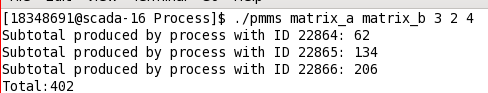
\includegraphics[width=10cm]{process_maXmb.png}
  \caption{Example of multi-process variant of pmms running with test input
    matrix_a and matrix_b.}
  \label{fig:example}
\end{figure}
\\\\\\
Thread: \begin{figure}[!htb]
  \centering
  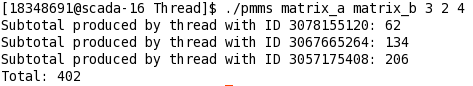
\includegraphics[width=10cm]{thread_maXmb.png}
  \caption{Example of multi-threaded variant of pmms running with test input
            matrix\_a and matrix\_b.}
  \label{fig:example}
\end{figure}
\\\\\\
\subsubsection{\it matrix\_E \times matrix\_F}
expected result = \begin{bmatrix}
44222 &38629 &383427& 39909& 37049 &35001 &44581& 38219& 22407 &40499\\
30575& 22032 &28715 &30681 &28734 &27747 &28599 &25073 &18021 &27677\\
32191 &25793 &26779& 27982 &32055 &23168 &31030 &24742 &16520 &31244\\
34988 &30154 &32111 &32173 &33867 &26767 &35108 &33353 &17498 &34180\\
32298 &27443 &27625 &31489 &27763 &32185 &30499 &28208 &20311 &32365\\
23632 &19850 &17870 &22325 &20858 &18773 &21604 &21496 &12184 &25428\\
31367 &25010 &28421 &30852 &25285 &27979 &32694 &22194 &16982 &23662\\
42105 &31006 &30561 &42201 &39686 &32411 &42447 &31343 &20263 &37789\\
43968 &31550 &36839 &40589 &39505 &35296 &39949 &36410 &25311 &42319\\
24443 &17542 &23493 &25206 &21177 &18961 &23309 &22632 &13229 &21501
\end{bmatrix}
\\\\\\
expected subtotals = \begin{bmatrix}
                    378858\\
                    267854\\
                	271504\\
                    310199\\
                    	290186\\
                        	204020\\
            	264446\\
                	349812\\
                    371736\\
                    	211493\\
                    \end{bmatrix}
\\\\\\
expected total = 2920108
\\\\\\
\textbf{Results}:
\\\\
Process:
\begin{figure}[!htb]
  \centering
  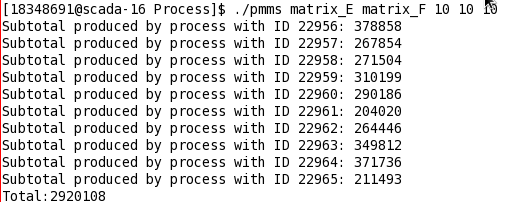
\includegraphics[width=10cm]{process_meXmf.png}
  \caption{Example multi-process variant of pmms running with test inputs
            matrix_E and matrix_F.}
  \label{fig:example}
\end{figure}
\\\\
Thread:
\begin{figure}[!htb]
  \centering
  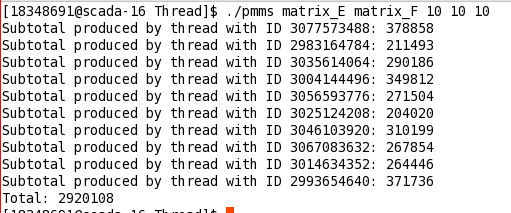
\includegraphics[width=10cm]{thread_meXmf.png}
  \caption{xample multi-threaded variant of pmms running with test inputs
            matrix_E and matrix_F.}
  \label{fig:example}
\end{figure}

\section{ReadMe}
\textbf{Purpose}\\
Matrix multiplication program using multiple processes and multiple threads
written in C99.
\\\\
The program prints out the subtotal calculated for each row along with the ID
of the thread/process that computed it. The total is then printed out after
all the rows have been calculated.
\\\\\\
\textbf{Files Included}
\begin{verbatim}
Process
    makefile
    pmms.c
    pmms.h

Thread
    makefile
    pmms.c
    pmms.h

Other
    test files
\end{verbatim}
\\\\\\
\textbf{Compile}
\begin{verbatim}
    make
\end{verbatim}
\\\\\\
\textbf{Execution}
\begin{verbatim}
    ./pmms matrix_one matrix_two M N K
\end{verbatim}
\\
matrix\_one = first matrix file\\
matrix\_two = second matrix file\\
M = matrix one columns\\
N = matrix one rows/matrix two cols\\
K = matrix two rows\\

%%%%%%%%%%%%%%%%%%%%%%%%%%%%%%%%%%%%%%%%%%%%%%%%%%%%%%%%%%%%%%%%%%%%%%
%% Finally we specify the format required for our references and the
%% name of the bibtex file where our references should be taken from.
%%%%%%%%%%%%%%%%%%%%%%%%%%%%%%%%%%%%%%%%%%%%%%%%%%%%%%%%%%%%%%%%%%%%%%

\bibliographystyle{plainnat}
\bibliography{example}

\end{document}

%%%%%%%%%%%%%%%%%%%%%%%%%%%%%%%%%%%%%%%%%%%%%%%%%%%%%%%%%%%%%%%%%%%%%%
%% The end.
%%%%%%%%%%%%%%%%%%%%%%%%%%%%%%%%%%%%%%%%%%%%%%%%%%%%%%%%%%%%%%%%%%%%%%
